\documentclass[10pt]{article}

\usepackage[margin=0.72in]{geometry}
\usepackage{amsmath,amssymb}
\usepackage{booktabs}
\usepackage{tabularx}
\usepackage{xcolor}
\usepackage{tikz}
\usepackage{microtype}
\usepackage[hidelinks]{hyperref}

\hypersetup{
  pdftitle={Prism BA on Cold Production Problems: Muell and Fuchsberg},
  pdfauthor={Prism BA Research Project}
}

\setlength{\parindent}{0pt}
\setlength{\parskip}{0.55em}
\setlength{\tabcolsep}{4.5pt}
\renewcommand{\arraystretch}{1.12}
\newcolumntype{Y}{>{\raggedright\arraybackslash}X}
\definecolor{prism}{HTML}{2E6FBB}
\definecolor{caspar}{HTML}{D26A3A}
\definecolor{muted}{HTML}{6B7280}

\newcommand{\hbarplot}[6]{%
  \begin{tikzpicture}[x=#5cm,y=0.62cm]
    \draw[gray!35] (0,-0.35) -- (#4,-0.35);
    \foreach \x in {0,#6,...,#4} {
      \draw[gray!20] (\x,-0.25) -- (\x,1.65);
      \node[font=\scriptsize,gray] at (\x,-0.58) {\x};
    }
    \fill[prism] (0,0) rectangle (#2,0.42);
    \fill[caspar] (0,0.82) rectangle (#3,1.24);
    \node[anchor=east,font=\small] at (-0.2,0.21) {Prism};
    \node[anchor=east,font=\small] at (-0.2,1.03) {Caspar};
    \node[anchor=west,font=\small] at (#2+0.25,0.21) {#2 s};
    \node[anchor=west,font=\small] at (#3+0.25,1.03) {#3 s};
    \node[anchor=west,font=\bfseries\small] at (0,1.78) {#1};
  \end{tikzpicture}%
}

\title{\vspace{-1.4em}\textbf{Prism BA on Cold Production Problems}\\
\large Muell and Fuchsberg measurements against Caspar}
\author{Prism BA Research Project\\\small Evidence report; frozen numbers, mixed-configurations labelled explicitly}
\date{13 September 2026}

\begin{document}
\maketitle

\begin{abstract}
This report isolates the available cold, production-style bundle-adjustment evidence for Prism and Caspar.  The primary experiment uses one pre-registered Prism Config R on 22 Muell global-BA snapshots and five Fuchsberg dumps, with three repetitions per cell and solver clocks excluding input loading.  Endpoint quality is effectively tied: all 22 Muell cells are ties and all five Fuchsberg cells lie within $+0.077\%$ of Caspar.  Prism uses 31$\times$ less total solver wall on Muell and 12.1$\times$ less on Fuchsberg.  The convergence-rate comparison is subtler: Caspar reaches a coarse 1\% gap faster, while Prism is faster or tied near a 0.1\% gap.  A separate 8,788-camera, 16.75-million-observation measurement shows both measured Prism profiles beating Caspar FP32 and FP64 in endpoint and total wall.  These are strong fastest-among-tested production-workload results, but they do not establish a universal fastest-solver claim.
\end{abstract}

\section{What ``cold problems'' means here}

The cold set is distinct from the repeatedly tuned BAL photo-tourism panel.  It contains production global-BA states from two reconstruction workloads:

\begin{center}
\begin{tabularx}{0.96\linewidth}{lrrrrY}
\toprule
Family & Cells & Cameras & Observations & Repeats & Character \\
\midrule
Muell & 22 & 24--493 & 30K--314K & $N=3$ & Warm, well-conditioned in-mapper global-BA snapshots from a production scan. \\
Fuchsberg & 5 & 526--8,788 & 1.08M--16.75M & $N=3$ & Large monocular conversion/global-BA dumps, including the largest production problem in this ledger. \\
\bottomrule
\end{tabularx}
\end{center}

The primary ledger fixes Config R before the sweep.  Prism and Caspar use their own native solve clocks with loading excluded.  Endpoint comparisons use a $\pm0.01\%$ tie band where a win/tie count is reported; the Fuchsberg family statement instead reports the observed worst endpoint difference.  Total-wall ratios compare completed configured budgets and therefore must be accompanied by time-to-gap measurements.

\section{Primary cold-workload result: pre-registered Config R}

\begin{center}
\begin{tabularx}{0.98\linewidth}{lrrrrY}
\toprule
Family & Quality result & Worst reported gap & Total wall ratio & 1\% gap ratio & 0.1\% gap ratio \\
\midrule
Muell & 22/22 ties & median $-0.0000\%$ & $31.0\times$ & $1.08\times$ & $2.62\times$ \\
Fuchsberg & 5/5 within tolerance & $+0.077\%$ & $12.1\times$ & $0.54\times$ & $1.01\times$ \\
\bottomrule
\end{tabularx}
\end{center}

All ratios in the last three columns are Caspar time divided by Prism time.  A value greater than one favours Prism.  Thus Prism has the lower configured total wall on both families.  At a coarse 1\% gap, Muell is roughly tied and Caspar is faster on Fuchsberg.  At a tight 0.1\% gap, Prism is 2.62$\times$ faster on Muell and statistically tied in rate on Fuchsberg.  This is why the report does not use Caspar's long post-convergence crawl to claim a large time-to-equal-quality speedup.

\begin{figure}[h]
\centering
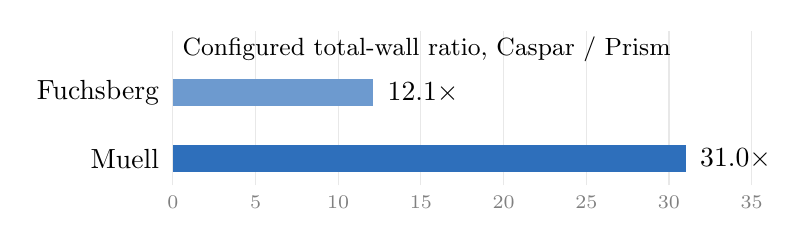
\begin{tikzpicture}[x=0.21cm,y=0.70cm]
  \foreach \x in {0,5,...,35} {
    \draw[gray!18] (\x,-0.25) -- (\x,2.55);
    \node[font=\scriptsize,gray] at (\x,-0.55) {\x};
  }
  \fill[prism] (0,0) rectangle (31,0.48);
  \fill[prism!70] (0,1.20) rectangle (12.1,1.68);
  \node[anchor=east] at (-0.25,0.24) {Muell};
  \node[anchor=east] at (-0.25,1.44) {Fuchsberg};
  \node[anchor=west,font=\bfseries] at (31.3,0.24) {$31.0\times$};
  \node[anchor=west,font=\bfseries] at (12.4,1.44) {$12.1\times$};
  \node[anchor=west,font=\small] at (0,2.22) {Configured total-wall ratio, Caspar / Prism};
\end{tikzpicture}
\caption{Total configured solver wall.  These ratios include Caspar's late crawl and are not, by themselves, convergence-rate ratios.}
\end{figure}

\begin{figure}[h]
\centering
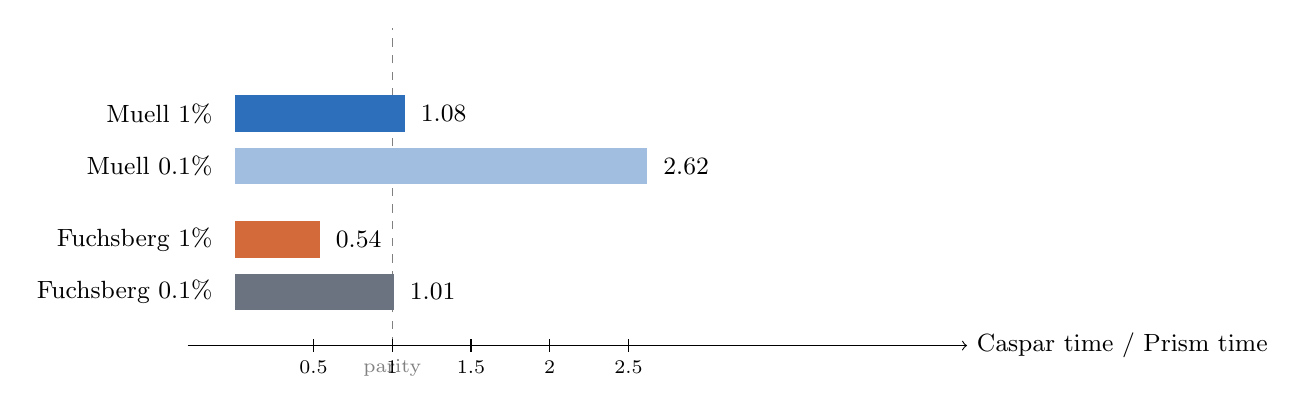
\begin{tikzpicture}[x=2.0cm,y=1.55cm]
  \draw[->] (-0.3,0) -- (4.65,0) node[right,font=\small] {Caspar time / Prism time};
  \draw[gray,dashed] (1,0) -- (1,2.6);
  \node[font=\scriptsize,gray] at (1,-0.18) {parity};
  \foreach \x/\lab in {0.5/0.5,1/1,1.5/1.5,2/2,2.5/2.5} {
    \draw (\x,-0.05) -- (\x,0.05);
    \node[font=\scriptsize] at (\x,-0.18) {\lab};
  }
  \fill[prism] (0,1.75) rectangle (1.08,2.05);
  \fill[prism!45] (0,1.32) rectangle (2.62,1.62);
  \fill[caspar] (0,0.72) rectangle (0.54,1.02);
  \fill[muted] (0,0.29) rectangle (1.01,0.59);
  \node[anchor=east,font=\small] at (-0.08,1.90) {Muell 1\%};
  \node[anchor=east,font=\small] at (-0.08,1.47) {Muell 0.1\%};
  \node[anchor=east,font=\small] at (-0.08,0.87) {Fuchsberg 1\%};
  \node[anchor=east,font=\small] at (-0.08,0.44) {Fuchsberg 0.1\%};
  \node[anchor=west,font=\small] at (1.12,1.90) {1.08};
  \node[anchor=west,font=\small] at (2.66,1.47) {2.62};
  \node[anchor=west,font=\small] at (0.58,0.87) {0.54};
  \node[anchor=west,font=\small] at (1.05,0.44) {1.01};
\end{tikzpicture}
\caption{Descent-rate view.  The apparent 12--31$\times$ total-wall advantage contracts sharply when both solvers are compared at the same quality gap.}
\end{figure}

\section{Largest measured cold problem: Fuchsberg \texttt{gba\_234}}

The largest single problem has 8,788 cameras and 16.75 million observations.  The table below is a separate measured configuration comparison retained from the production ledger; it is not Config R and is therefore not pooled into the preceding family tally.

\begin{center}
\begin{tabular}{lrrr}
\toprule
Solver/configuration & Final cost & Native wall (s) & Caspar-FP64 wall / wall \\
\midrule
Prism fast & $3.0012\times10^7$ & 49.7 & $5.1\times$ \\
Prism all-on & $3.0017\times10^7$ & 27.5 & $9.2\times$ \\
Caspar FP32 & $3.0037\times10^7$ & 95.0 & $2.7\times$ \\
Caspar FP64 & $3.0019\times10^7$ & 252.0 & $1.0\times$ \\
\bottomrule
\end{tabular}
\end{center}

Both measured Prism profiles finish below both Caspar endpoints and use less wall.  ``All-on'' is faster than ``fast'' in this row because these names identify frozen profiles rather than an ordering guaranteed on every problem.

\begin{figure}[h]
\centering
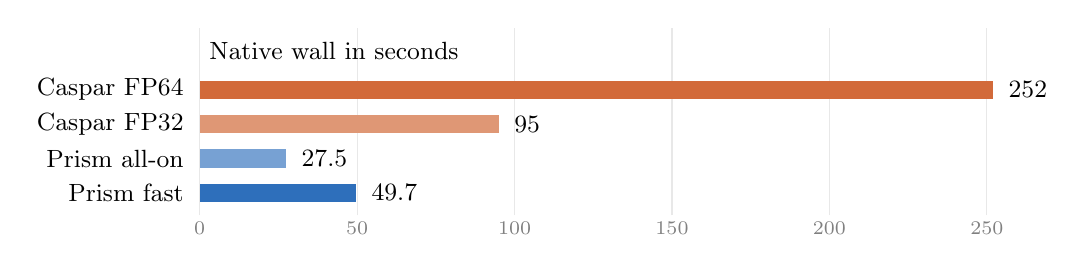
\begin{tikzpicture}[x=0.040cm,y=0.58cm]
  \foreach \x in {0,50,...,250} {
    \draw[gray!18] (\x,-0.3) -- (\x,3.8);
    \node[font=\scriptsize,gray] at (\x,-0.58) {\x};
  }
  \fill[prism] (0,0) rectangle (49.7,0.40);
  \fill[prism!65] (0,0.75) rectangle (27.5,1.15);
  \fill[caspar!70] (0,1.50) rectangle (95,1.90);
  \fill[caspar] (0,2.25) rectangle (252,2.65);
  \node[anchor=east,font=\small] at (-2,0.20) {Prism fast};
  \node[anchor=east,font=\small] at (-2,0.95) {Prism all-on};
  \node[anchor=east,font=\small] at (-2,1.70) {Caspar FP32};
  \node[anchor=east,font=\small] at (-2,2.45) {Caspar FP64};
  \node[anchor=west,font=\small] at (51.5,0.20) {49.7};
  \node[anchor=west,font=\small] at (29.3,0.95) {27.5};
  \node[anchor=west,font=\small] at (96.8,1.70) {95};
  \node[anchor=west,font=\small] at (253.8,2.45) {252};
  \node[anchor=west,font=\small] at (0,3.30) {Native wall in seconds};
\end{tikzpicture}
\caption{Configured wall on the 8,788-camera Fuchsberg problem.}
\end{figure}

\section{End-to-end Muell mapper result}

A separate N=3 interleaved incremental-mapping experiment measures the full application rather than isolated BA calls.  Prism completes in 1,051 seconds versus 1,174 seconds for Caspar, a 10.5\% end-to-end reduction with non-overlapping measured ranges.  Both reconstruct all 493 registered images, with final reprojection error between 1.1099 and 1.1107 pixels.  The isolated BA phase accounts for the difference: 167.4 seconds for Prism versus 286.4 seconds for Caspar, a 41.6\% reduction over approximately 48--50 BA calls.  Non-BA work agrees within 0.7\%.

\begin{center}
\hbarplot{End-to-end mapper}{1051}{1174}{1200}{0.011}{200}
\end{center}

\begin{center}
\hbarplot{Accumulated BA phase}{167.4}{286.4}{300}{0.044}{50}
\end{center}

This is the strongest application-level cold result because it includes the consequences of solver choices on the surrounding mapper trajectory.  It should be reported together with the equal map registration and reprojection statistics.

\section{Independent Muell-gba146 target audit}

The largest Muell snapshot has 493 cameras, 313,987 points and 2,118,671 observations.  Its independently checked initial cost is 2,442,177.030208.  A later Eta2/B6v7 run registered the target $1,946,488.7463$ and reached it in all three repetitions at a median 4.0303 seconds (range 4.0263--4.0376), finishing at median cost 1,946,467.1524 after 16 outer iterations, zero rejects and 980 Schur products.

The separately frozen 90-second Caspar audit used the same input hash and independent FP64 rescoring:

\begin{center}
\begin{tabular}{lrrrr}
\toprule
Arm & Hits & Median audited cost & Median wall (s) & Median accepts / rejects \\
\midrule
Prism Eta2/B6v7 & 3/3 & 1,946,467.15 & 4.030 & 16 / 0 \\
Caspar FP32 & 0/3 & 1,961,895.56 & 90.006 & 960 / 682 \\
Caspar FP64 & 0/3 & 1,962,982.12 & 90.145 & 568 / 0 \\
\bottomrule
\end{tabular}
\end{center}

This row shows a target that Caspar does not reach under its 90-second caps, so it supports a quality-and-budget statement rather than a finite time-to-target speed ratio.  The FP32 median happens to be below the FP64 median by 0.055\%; that difference is small relative to the distance to the registered target and should not be interpreted as a general precision ordering.

\section{Claim boundary and missing evidence}

The cold evidence supports the following wording:

\begin{quote}
On the measured Muell and Fuchsberg production workloads, Prism matches Caspar's endpoint quality while reducing configured solver wall substantially.  At identical quality gaps the advantage is workload- and tolerance-dependent: Prism is strongest near tight convergence on Muell, while Caspar reaches coarse accuracy faster on the largest Fuchsberg sequence.  On the 8,788-camera measured configuration, Prism beats Caspar FP32 and FP64 in both endpoint and total wall.
\end{quote}

It does not support ``fastest BA solver'' without qualification.  The available local archive lacks the per-iteration Fuchsberg traces behind the five-cell aggregate, so this report includes summary figures rather than reconstructed convergence curves for those dumps.  The raw Muell-gba146 Caspar rows are available and independently audited, but they use a different stopping budget from the Config-R family sweep.  Future publication should restore the raw Fuchsberg traces, retain binary and input hashes per cell, and plot actual target crossings rather than infer them from total budgets.

\section*{Provenance}

Primary Config-R family numbers and the total-wall/descent-rate correction come from \texttt{REPRODUCE.md}, Section 6c, in the synchronized research tree.  The additional \texttt{gba\_234} and end-to-end mapper rows come from the corrected product-workload section of \texttt{docs/results\_2026\_09.md}.  The Muell-gba146 Caspar audit comes from \nolinkurl{/workspace/prism-muell-caspar/summary.json}; the Eta2/B6v7 row comes from \nolinkurl{research/eta2_wave5/b6v7-muell-summary.json}.  No number in this report was inferred from a plot.

\end{document}
